%% PODSTAWOWE USTAWIENIA DOKUMENTU
\documentclass[12pt, a4paper, polish]{article}
\DeclareUnicodeCharacter{2003}{-}
%\usepackage[a4paper, lmargin=2.5cm, rmargin=2.5cm, hmargin=2.5cm, bmargin=2.5cm]{geometry}
\usepackage[a4paper,top=2.5cm,bottom=1.5cm,left=1.5cm,right=1.5cm]{geometry}
%\geometry{verbose,lmargin=2.5cm,rmargin=2.5cm}
\usepackage{enumerate}
% Symbole matematyczne
\usepackage{latexsym}
% Formatowanie czcionki
\usepackage[T1]{fontenc}
% Formatowanie polskich znaków
\usepackage{polski}
\usepackage[utf8]{inputenc}
% Akapit po sekcji
%\usepackage{indentfirst}
% Ustawienie nagłówków i stopek
\usepackage{fancyhdr}
% Liczba stron
\usepackage{lastpage}
% Kolumny
\usepackage{paracol}
% Czcionka latin modern
\usepackage{lmodern}
% Równania matematyczne
\usepackage{amsmath}
\usepackage{amsfonts}
\usepackage{amssymb}
\usepackage{amsthm}
% Wstawianie grafik
\usepackage{graphicx}
\usepackage[section]{placeins} % Ogarnięcie obrazków
\usepackage{subcaption}

%% ODSTĘPY W WIERSZACH
\setlength{\parindent}{2cm}
\setlength{\parskip}{0.1cm}
\linespread{1}

%% SZARE TŁO TEKSTU
\usepackage[most]{tcolorbox}
\tcbset{
    frame code={}
    center title,
    left=0pt,
    right=0pt,
    top=0pt,
    bottom=0pt,
    colback=gray!30,
    colframe=white,
    width=\dimexpr\textwidth\relax,
    enlarge left by=0mm,
    boxsep=5pt,
    arc=0pt,outer arc=0pt,
    }

% HIPERŁĄCZA SPISU TREŚCI
\usepackage{hyperref}
\hypersetup{
    colorlinks,
    citecolor=black,
    filecolor=black,
    linkcolor=black,
    urlcolor=black
}

\begin{document}
\fancyhf{}	% Usunięcie domyślnego stylu numerowania

% ********************** TYTUŁ ****************************
\noindent\textsf{\begin{Large}Laboratorium Sterowania Robotów Manipulacyjnych \\\end{Large}
Raport z ćwiczeń\textbf{ Z7, Z8}\\
Szymon Kacperek, Adrianna Kręglewska, Adam Banaszczyk\\
AiR, studia stacjonarne II stopnia,  specjalność SSiR, rok akademicki 2019/2020\\
\rule{\columnwidth}{0.2pt}}

\thispagestyle{empty}
\pagestyle{fancy}
\fancyhead{}
\rhead{\thepage}
\renewcommand{\headrulewidth}{0pt}%{}
\setlength{\footskip}{1mm}

%							*****************POCZĄTEK DOKUMENTU*****************
\section{Sterowanie w podprzestrzeni typu \textit{hiperkula}}
	Dla modelu manipulatora PM2R z silnikami zaprojektowany został regulator ROOS dla ograniczonej podprzestrzeni sterowań: hiperkuli. Układ sterowania wyrażony jest wprost dla napięć wraz ze wzmacniaczem mocy, ograniczającym napięcia zasilania dla obu silników. Symulacje przebiegają dla zerowych warunków początkowych (manipulator wyprostowany w prawo).

	Z założeń wynika, iż regulator ROOS jest odporny na nieznajomość strukturalną i parametryczną modelu, zatem dla celów symulacji wprowadzono niepewności parametryczne: 10\% dla długości pierwszego oraz drugiego ramienia oraz 10\% dla masy drugiego ramienia. Silnik został zamodelowany według danych \textit{maxon DC motor FF2260, 883} oraz dwóch przekładni \textit{110507} o przełożeniu $\eta=1/181$. Wartości współczynników diagonalnych macierzy wzmocnień dla $\epsilon=5,4$ przyjęto eksperymentalnie:
	$$
	\Lambda=\begin{bmatrix} 3,5 & 0 \\0 & 3,6 \end{bmatrix}, \quad  D=\begin{bmatrix} 2,25 & 0 \\0 & 2,35 \end{bmatrix}
	$$

\subsection{Wnioski}
	Mimo niepewności parametrycznej, odpowiedź modelu manipulatora odwzorowuje zadane wartości referencyjne. Z naszych obserwacji wynika, iż zjawisko \textit{chatteringu}  występuje zawsze - jest intensywniejsze, gdy różnica między wartością współczynnika $\epsilon$ oraz współczynnikami diagonalnych macierzy wzmocnień jest mniejsza, natomiast w przypadku, gdy współczynnik $\epsilon=0$  lub jest mniejszy od współczynników diagonalnych macierzy wzmocnień, zjawisko \textit{chatteringu} znacznie się intensyfikuje.
	
	Zasadniczym ograniczeniem tego układu jest ograniczenie napięcia sterującego $u_{HKmax}$ widoczne na rys. 1a, sygnał sterujący bazuje na najmniejszym z ograniczeń.
\subsection{Prezentacja wyników}
\begin{figure}[h]\centering
		a) 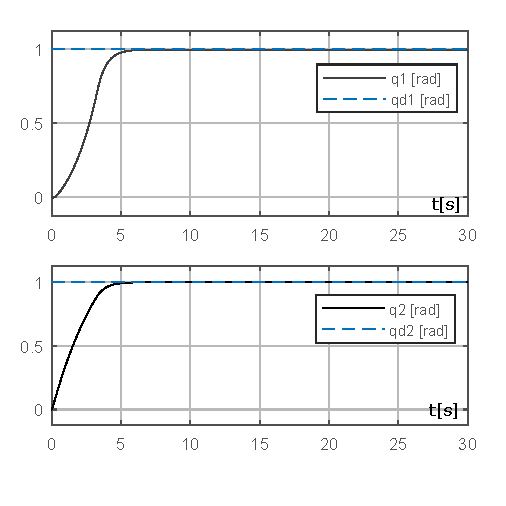
\includegraphics[width=0.30\columnwidth]{SRManL4_ZADANIE1/figs/01_POZYCJE_e5.4_uHKmax12} b)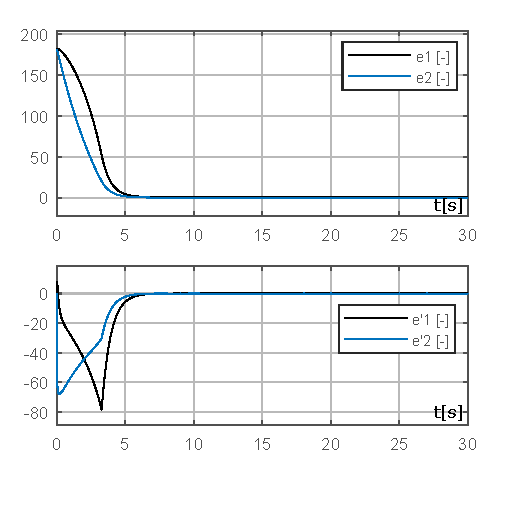
\includegraphics[width=0.30\columnwidth]{SRManL4_ZADANIE1/figs/01_UCHYBY_e5.4_uHKmax12} c)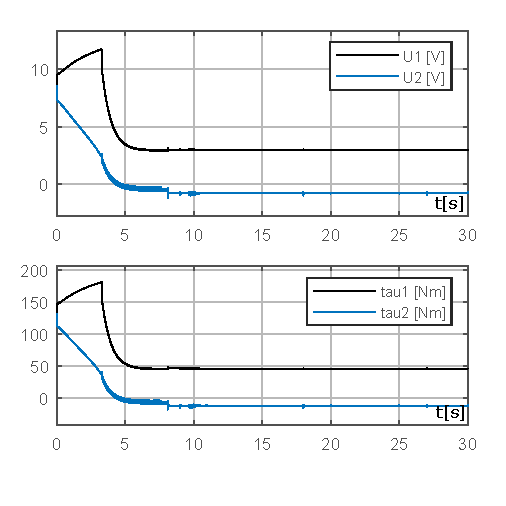
\includegraphics[width=0.30\columnwidth]{SRManL4_ZADANIE1/figs/01_SYGNALY_e5.4_uHKmax12}\caption{
			Wyniki symulacji dla $u_{HKmax}=12$ [V] o wymuszeniu $Q_d=[1\quad1]$: przebiegi a) pozycji ogniw wraz z zadanym sygnałem referencyjnym, b) uchybów pozycji i prędkości, c)  napięć sterujących oraz odpowiadające im momenty generowane na wałach silników.}
\end{figure}
\begin{figure}[!ht]\centering
	a) 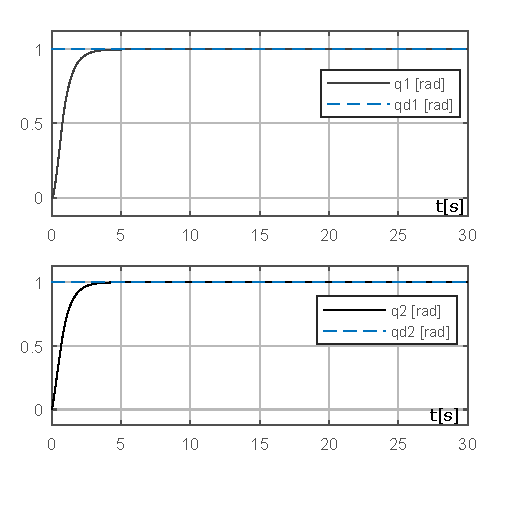
\includegraphics[width=0.30\columnwidth]{SRManL4_ZADANIE1/figs/02_POZYCJE_e5.4_uHKmax24} b)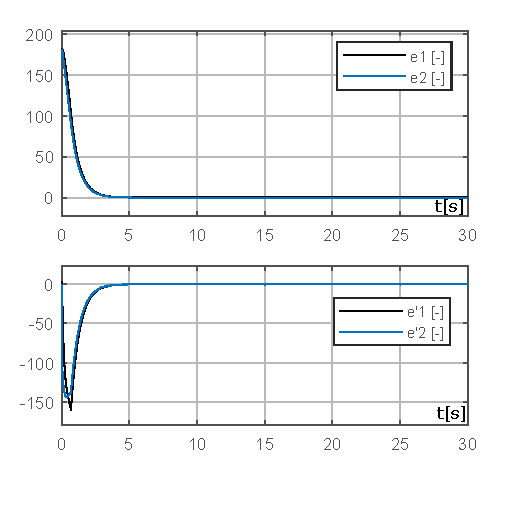
\includegraphics[width=0.30\columnwidth]{SRManL4_ZADANIE1/figs/02_UCHYBY_e5.4_uHKmax24} c)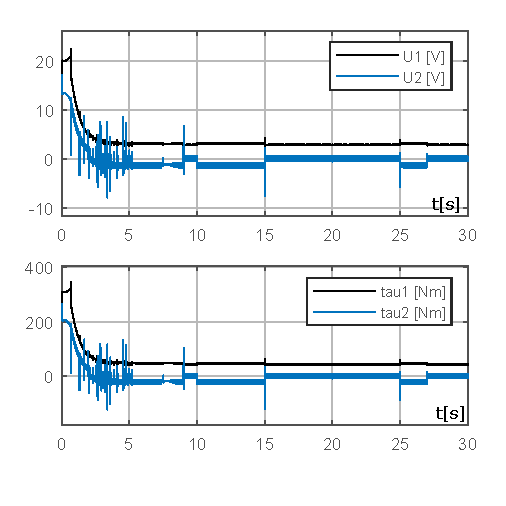
\includegraphics[width=0.30\columnwidth]{SRManL4_ZADANIE1/figs/02_SYGNALY_e5.4_uHKmax24}\\
	d) 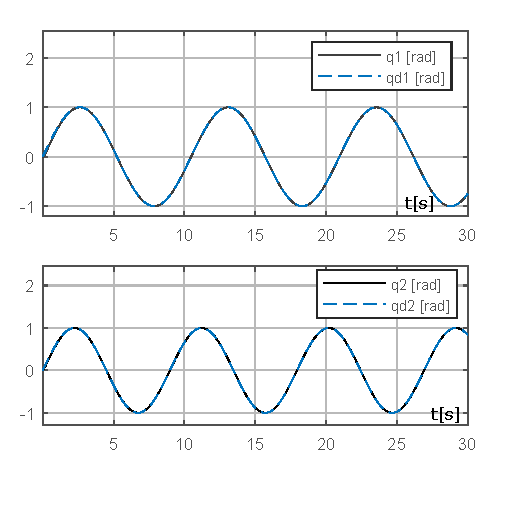
\includegraphics[width=0.30\columnwidth]{SRManL4_ZADANIE1/figs/03_POZYCJE_e5.4_uHKmax24} e)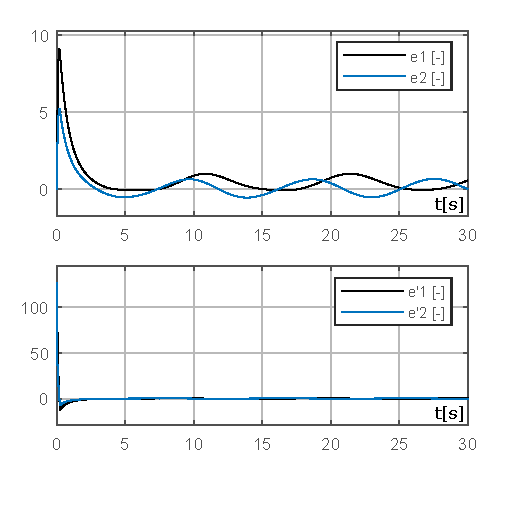
\includegraphics[width=0.30\columnwidth]{SRManL4_ZADANIE1/figs/03_UCHYBY_e5.4_uHKmax24} f)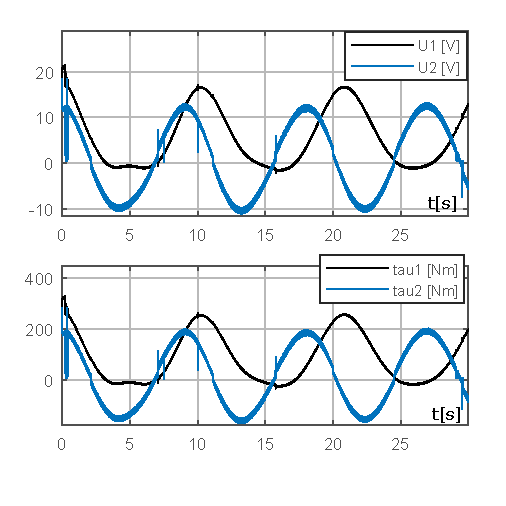
\includegraphics[width=0.30\columnwidth]{SRManL4_ZADANIE1/figs/03_SYGNALY_e5.4_uHKmax24}\\
	g) 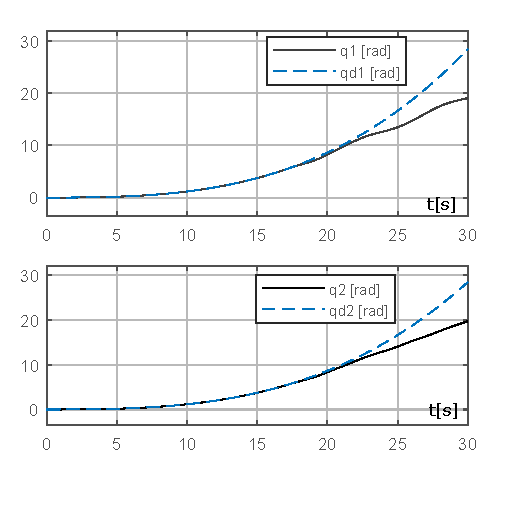
\includegraphics[width=0.30\columnwidth]{SRManL4_ZADANIE1/figs/04_POZYCJE_e5.4_uHKmax24} h)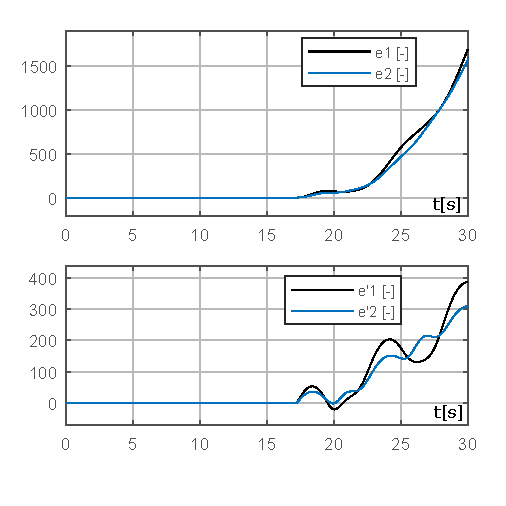
\includegraphics[width=0.30\columnwidth]{SRManL4_ZADANIE1/figs/04_UCHYBY_e5.4_uHKmax24} i)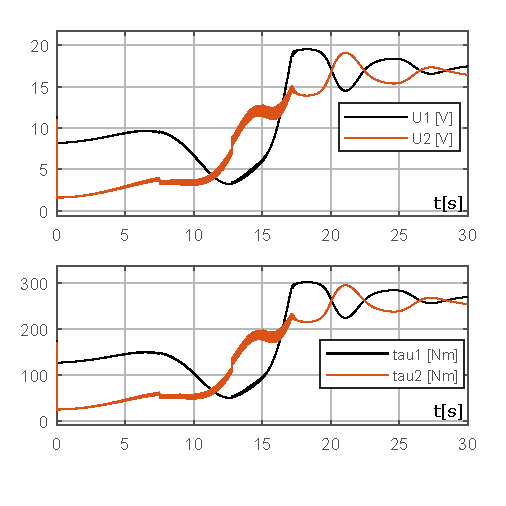
\includegraphics[width=0.30\columnwidth]{SRManL4_ZADANIE1/figs/04_SYGNALY_e5.4_uHKmax24}\caption{
		Wyniki symulacji dla $u_{HKmax}=24$ [V]. Przebiegi a) pozycji ogniw wraz z zadanym sygnałem referencyjnym, b) uchybów pozycji i prędkości, c)  napięć sterujących oraz odpowiadające im momenty generowane na wałach silników, o wymuszeniu:\\
		 \textbf{a-c:} $Q_d=[1\quad1]$;\\
		 \textbf{d-f:} $Q_d=[\sin(0,6t);\quad \sin(0,7t)]$;\\
		 \textbf{g-i:} $Q_d=[0,0025t^3+0,0020t^2+0,0015t+0,001]$.}
\end{figure}

\section{Sterowanie w podprzestrzeni typu \textit{hiperprostopadłościan}}
\end{document}
